% https://www.overleaf.com/latex/templates/sprint-beyond-the-book-template/kgckkccxfxcj
% 這份報告是用上面網址裡的資料建立的

\documentclass[nols]{tufte-book}
%\documentclass{tufte-handout}
\usepackage[caption=false]{subfig}

\usepackage{booksprint}

\usepackage{pdflscape}

\setcounter{secnumdepth}{3}
\setcounter{tocdepth}{2}

\usepackage{fancyhdr}
% 加上 table in the header 
% https://tex.stackexchange.com/questions/113240/tables-as-header-and-footer

\usepackage{hyperref} %加入 hyperlink

\usepackage{natbib}

%\usepackage[utf8]{inputenc}
\usepackage[T1]{fontenc}
\usepackage{fontspec}
\renewcommand{\allcapsspacing}[1]{{\addfontfeature{LetterSpace=10.0}#1}}
\renewcommand{\smallcapsspacing}[1]{{\addfontfeature{LetterSpace=5.0}#1}}
\renewcommand{\textsc}[1]{\smallcapsspacing{\textsmallcaps{#1}}}
\renewcommand{\smallcaps}[1]{\smallcapsspacing{\scshape\MakeTextLowercase{#1}}}
% https://www.overleaf.com/latex/examples/demonstration-of-noto-serif-cjk-and-noto-sans-cjk-fonts/sgrwgcddtqsq
\usepackage{setspace}


%set-up 中文環境
\usepackage[CJKspace]{xeCJK}
\usepackage{xpinyin}

\setmainfont{Noto Serif Light}
\setsansfont{Noto Sans}
\setmonofont[Scale=MatchLowercase]{Noto Mono}

\setCJKmainfont{Noto Serif CJK TC}
\setCJKsansfont{Noto Sans CJK TC}
\setCJKmonofont{Noto Sans Mono CJK TC}


%表格
\usepackage{amsmath}
\usepackage{amssymb}
\usepackage{hyperref}
\usepackage{array}

\usepackage{tabularx}
\usepackage{multirow}

\usepackage{ragged2e}
\usepackage{longtable}




\title[教學部跨領域案例討論集]{
\textbf{教學部\\
新竹臺大分院醫學中心 \\ 
教育推廣手冊}}
\author{教學部暨跨領域教學團隊}
\date{\today}

%\logos



\begin{document}
\maketitle
\tableofcontents



\onehalfspacing

\chapter{背景}

\section{跨領域討論會在新竹的歷史}

\subsection{我們為什麼要編這本手冊}

\section{2024年度會議回顧}

\begin{figure}
    \centering
    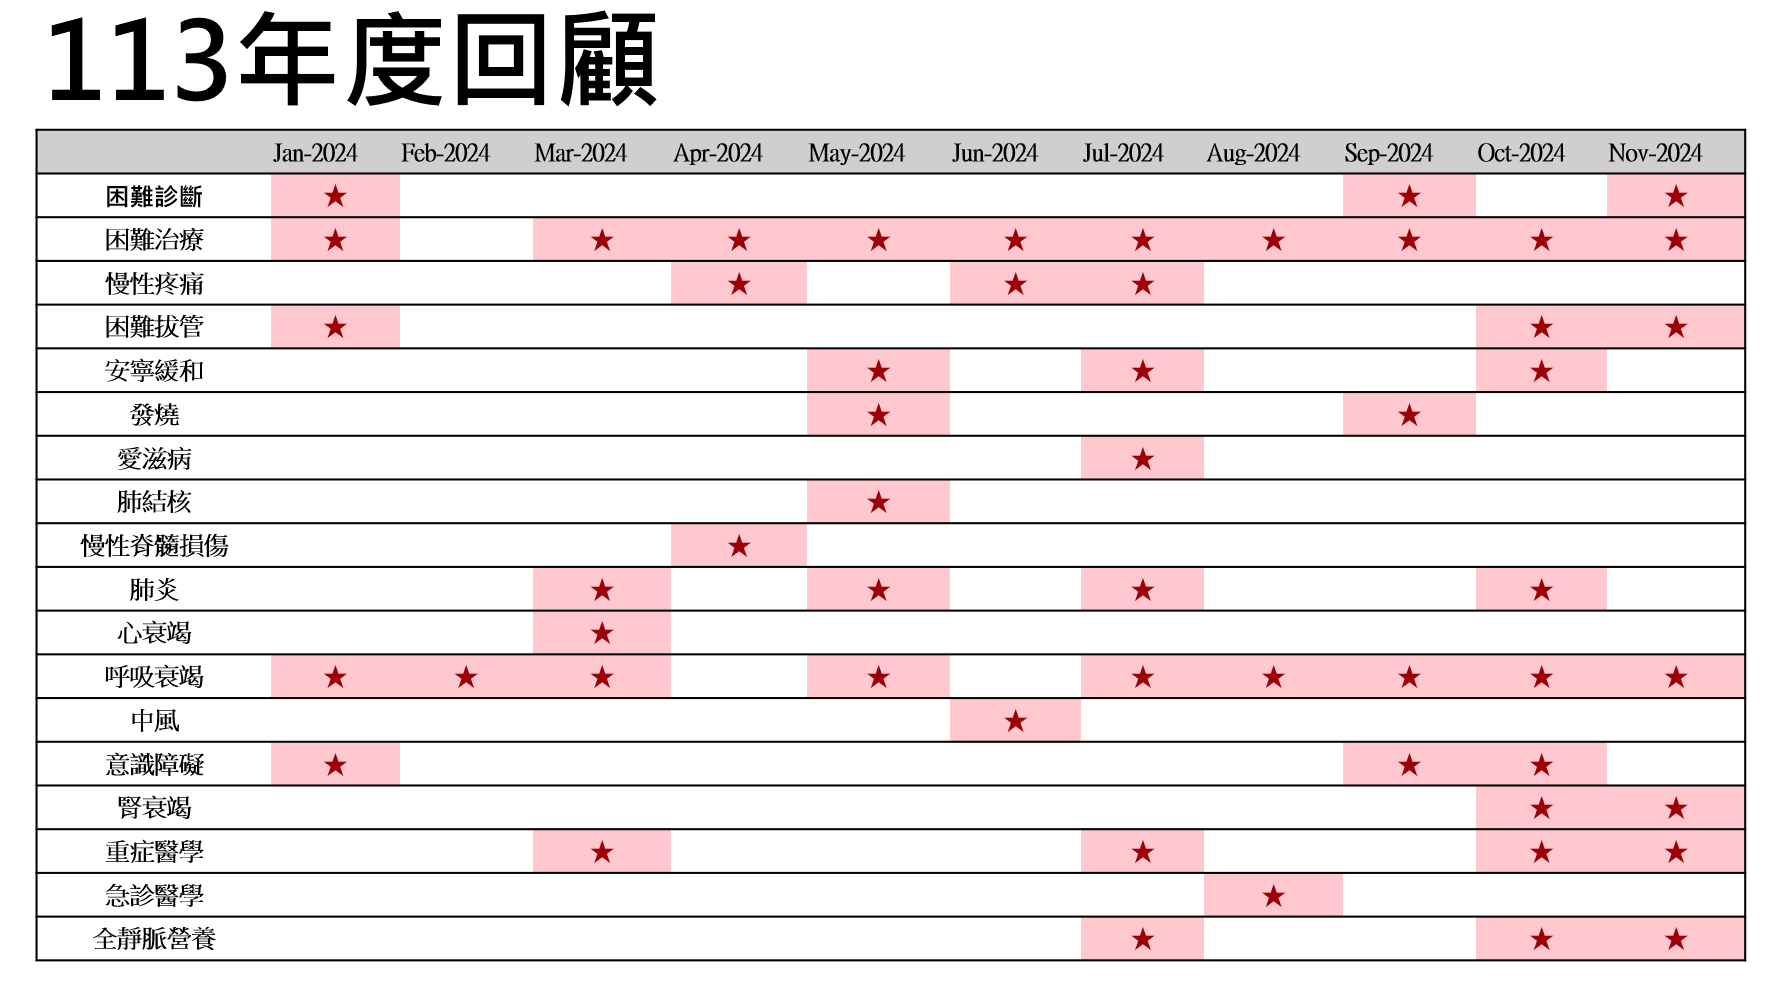
\includegraphics[width=0.75\linewidth]{images/edu/fig edu 2024 MDTD.png}
    \caption{Enter Caption}
    \label{fig:enter-label}
\end{figure}


\begin{longtable}{p{2cm}p{5cm}p{8cm}}
    \hline
    \textbf{日期} & \textbf{團隊} & \textbf{個案簡介與討論重點} \\
    \hline
    \endfirsthead

    \hline
    \textbf{日期} & \textbf{團隊} & \textbf{個案簡介與討論重點} \\
    \hline
    \endhead

    \hline
    \endfoot

    \hline
    \endlastfoot

    1/16 & 雲林台大分院跨領域團隊 & 38 歲女性，發生不明目擊的暈倒，持續 10 分鐘。 \\
    \hline
    2/20 & 生醫竹東呼吸照護病房團隊 & 66 歲女性，呼吸器依賴，轉至 RCW 接受呼吸訓練。 \\
    \hline
    3/19 & 雲林台大分院跨領域團隊 & 71 歲女性，過去兩週逐漸出現呼吸困難。 討論：冠心病合併心衰竭及肺炎的照護。 \\
    \hline
    4/16 & 生醫竹東護理之家團隊 & 38 歲男性，因脊椎壓迫導致下半身無知覺，無法行動，期望繼續復健治療。 討論：協助年輕脊髓損傷個案重建生活目標。 \\
    \hline
    5/21 & 雲林台大分院跨領域團隊 & 65 歲長期臥床男性，護理之家轉入急診，發現低血糖及低血氧，送入 ICU。X-ray 顯示右側肋膜積水。 討論：確定診斷為結核病 (TB)，護理之家照護重點及 TB 診斷困難。 \\
    \hline
    6/18 & 神骨復影醫個案討論團隊 & 72 歲男性，2023 年 10 月 9 日罹患右側橋腦中風，住院期間病人主訴雙側肩膀與雙側膝蓋疼痛，術後仍有關節疼痛。 討論：中風後合併關節疼痛的全人照護。 \\
    \hline
    7/16 & 雲林台大分院跨領域團隊 & 71 歲男性，定期進行愛滋病治療，新診斷膽管癌，住院化療後合併肺動脈栓塞。 \\
    \hline
    8/20 & 急診醫學部跨領域團隊 & 64 歲女性，機車事故，胸口撞擊龍頭，呼吸困難及胸痛。 討論：急診插管病人是否需要鎮靜藥物使用？ \\
    \hline
    9/24 & 雲林台大分院跨領域團隊 & 68 歲男性，失智症、第二型糖尿病、癲癇及高血脂，發燒持續一天。 討論：疱疹病毒性腦炎 (HSV 腦炎) 的診斷與治療。 \\
    \hline
    10/15 & 生醫竹北加護病房團隊 & 56 歲男性，腹痛三天內進展至多重器官衰竭。 討論：重症胰臟炎的診斷與治療困難。 \\
    \hline
    11/19 & 雲林台大分院跨領域團隊 & 42 歲男性，腹痛及嘔吐 10 天，急診懷疑腸阻塞。 討論：急性腸缺血診斷與治療，個案為腸道靜脈栓塞所致腸缺血 (較少見)。 \\
    \hline
\end{longtable}

\section{年度回顧與檢討}
本年度的跨院跨領域討論會涵蓋了多種不同類型的臨床個案，從急診處置、加護病房管理、慢性病照護到中風與復健，顯示了不同醫療單位的合作與臨床思維交流。未來可持續優化病人轉介流程、提升診斷準確性，以及加強各職類間的協作與溝通。

\section{表格範例- 心衰竭用藥}

\renewcommand{\arraystretch}{1.3} % 增加行距，使表格更清晰

\begin{longtable}{p{4cm}p{6cm}p{6cm}}
    \hline
    \textbf{藥物} & \textbf{優點} & \textbf{副作用} \\
    \hline
    \endfirsthead

    \hline
    \textbf{藥物} & \textbf{優點} & \textbf{副作用} \\
    \hline
    \endhead

    \hline
    \endfoot

    \hline
    \endlastfoot

    \textbf{Beta-Blockers} & 
    - 減緩心跳 \newline
    - 減少心肌耗氧量 \newline
    - 降低心肌重塑 &
    - 心跳過慢 \newline
    - 氣管收縮 \\
    \hline

    \textbf{Statins} & 
    - 降血脂 \newline
    - 減少動脈粥狀硬化 &
    - 肝功能指數異常 \newline
    - 肌肉疼痛 \\
    \hline

    \textbf{Angiotensin Converting Enzyme Inhibitors / Angiotensin Receptor Blockers} & 
    - 血管舒張 \newline
    - 降低心肌重塑 &
    - 高血鉀 \newline
    - 初期 eGFR 下降 \\
    \hline

    \textbf{Angiotensin Receptor-Neprilysin Inhibitor} & 
    - 血管舒張 \newline
    - 降低心肌重塑 &
    - 高血鉀 \newline
    - 初期 eGFR 下降 \\
    \hline

    \textbf{Mineralocorticoid Receptor Antagonists} & 
    - 減少鈉離子、水滯留 \newline
    - 降低心肌重塑 &
    - 高血鉀 \newline
    - 男性女乳症 \\
    \hline

    \textbf{SGLT-2 Inhibitors} & 
    - 保護心臟、腎臟 &
    - 泌尿道感染 \newline
    - 初期 eGFR 下降 \\
    \hline

    \textbf{Loop Diuretics} & 
    - 增加水排除 &
    - 電解質異常（低血鉀、低血鎂、低血鈣） \\
    \hline

\end{longtable}

% The bibliography style.
\bibliographystyle{abbrv}
\bibliography{Reference}



\end{document}